%\documentclass{layout/tudelft-aiaa}
\documentclass[twocolumn]{tudelft-aiaa}

%% Additional packages
\usepackage[T1]{fontenc}
\usepackage[utf8]{inputenc}

\usepackage{xcolor}
\usepackage{courier}
\usepackage{xfrac}
\usepackage{amsmath}


% Wordle colors
\definecolor{k}{RGB}{121,124,126}
\definecolor{y}{RGB}{195,180,95}
\definecolor{g}{RGB}{129,170,105}
\definecolor{w}{RGB}{255,255,255}

\usepackage{graphicx} % Adding images
\usepackage{amsmath} % Mathematics
\usepackage{siunitx} % Various functions, e.g. \num{}
\usepackage{tabularx} % Additional functions to tables
\usepackage{subcaption} % Subfigures and subcaptions

%% Additional commands
\setlength{\nomitemsep}{-\parsep} % Reduce white space in nomenclature
\setlength{\bibsep}{1pt} % Reduce white space in references
\renewcommand{\deg}{\si{\degree}\xspace}

%%%%% Title %%%%%

\title{Solving Wordle Heuristically}

\author{\textbf{Daniel W. Dichter} --- Independent Researcher}
\affil{Cambridge, Massachusetts, U.S.A.\\daniel.w.dichter@gmail.com\\February 13, 2022}

\begin{document}

\AlwaysPagewidth{

\maketitle

%%%%% Abstract %%%%%

\begin{abstract}
\noindent \normalfont Wordle is a daily word game in which a player must guess a hidden five-letter word in six or fewer tries. After each guess, they get a color-coded response that indicates how close their guess was. This paper describes a solver that wins all 2,315 possible games, averaging a score of 3.594 with a standard deviation of 0.676. This is comparable to the current-best solvers, yet is achieved heuristically with many fewer calculations.

\end{abstract}

\vspace{3 mm}

}

%%%%% Main Body %%%%%

\section{Game Parameters}

Wordle has two dictionaries: 2,315 possible solutions, and 12,972 acceptable guesses.\cite{Wardle}\cite{Glaiel} Solutions are limited to commonly known, non-S-plural words. The default version of the game is assumed, wherein guesses need not be consistent with known information. Games are assumed to be mutually independent, and thereby the solver cannot recall previous solutions to reduce the set of initial words.

\section{Probability and Value}

A matrix $P$ measuring 26x5 is defined, reporting the probability of each letter $\alpha$ in each position $\rho$ of the solution. Guessing a tile that is already known to have zero or unity probability\footnote{Obtained directly by a gray or green tile, or indirectly by deduction.} provides no new information, or \emph{value}. Accordingly, maximum value must occur at some intermediate $p$ corresponding to minimum certainty. This is modeled as a transfer function relating probability $p$ to value $v$:

\begin{equation}
\label{equation_p_vs_v}
v(p) = \sin (\pi p) ^ {\sfrac{2}{3}} \hspace{2mm} \text{for} \hspace{2mm} 0 \leq p \leq 1
%v(p) = \bigg( \frac{1}{2} \sin \Big( 2 \pi (p - \sfrac{1}{4} ) \Big) + \sfrac{1}{2} \bigg) ^ {1/3}
\end{equation}

A value matrix $V$, also measuring 26x5, is then similarly defined. $P$ and $V$ are updated after every move as solutions are eliminated.

\section{Scoring and Guessing}

To score the overall value of a word, interactions between tiles are modeled with a set of heuristics, as follows.

A tile with non-unity probability captures the value of that letter in that position, and one-half the value of that letter in all other positions. This is modeled as a 5x5 weight matrix $W$ containing ones on the diagonal and one-half everywhere else; rows correspond to the tile being scored, and columns correspond to the position being evaluated.

Tiles that letter-match with other tiles in the same word reduce each other's value, as if by \emph{interference}. Similarly, when unity-probability occurs, tiles may return as yellow, indicating the already-known tile(s), thereby reducing their value, as if by \emph{occlusion}. These phenomena are modeled in a 5x5 quality matrix $Q$ given in Table \ref{table_Q_matrix} as a function of $q_m$, the quantity of letter-matching tiles, and $q_u$, the quantity of letter-matching unity-probability tiles. $Q$ is defined for each tile as the probability of not being occluded divided by the quantity of non-unity letter-matching tiles.

\begin{table}
\begin{centering}
\begin{tabular}{l r}
\bf{Game State} & \bf{Words Left}\\
\hline
\noalign{\vskip 2mm}
\noindent \vspace{0 mm} \texttt{\textcolor{white}{\textbf{\colorbox{k}{S}\hspace{1 mm}\colorbox{k}{O}\hspace{1 mm}\colorbox{k}{A}\hspace{1 mm}\colorbox{y}{R}\hspace{1 mm}\colorbox{y}{E}\hspace{1 mm}}}} & 2,315\\
\noindent \vspace{0 mm} \texttt{\textcolor{white}{\textbf{\colorbox{y}{D}\hspace{1 mm}\colorbox{k}{I}\hspace{1 mm}\colorbox{k}{N}\hspace{1 mm}\colorbox{g}{E}\hspace{1 mm}\colorbox{g}{R}\hspace{1 mm}}}} & 117\\
\noindent \vspace{0 mm} \texttt{\textcolor{white}{\textbf{\colorbox{k}{U}\hspace{1 mm}\colorbox{g}{L}\hspace{1 mm}\colorbox{k}{A}\hspace{1 mm}\colorbox{k}{M}\hspace{1 mm}\colorbox{k}{A}\hspace{1 mm}}}} & 3\\
\noindent \vspace{0 mm} \texttt{\textcolor{white}{\textbf{\colorbox{g}{E}\hspace{1 mm}\colorbox{g}{L}\hspace{1 mm}\colorbox{g}{D}\hspace{1 mm}\colorbox{g}{E}\hspace{1 mm}\colorbox{g}{R}\hspace{1 mm}}}} & 1\\
\noalign{\vskip 2mm}
\hline
\noalign{\vskip 2mm}
\noindent \vspace{0 mm} \texttt{\textcolor{white}{\textbf{\colorbox{g}{S}\hspace{1 mm}\colorbox{k}{O}\hspace{1 mm}\colorbox{k}{A}\hspace{1 mm}\colorbox{k}{R}\hspace{1 mm}\colorbox{k}{E}\hspace{1 mm}}}} & 2,315\\
\noindent \vspace{0 mm} \texttt{\textcolor{white}{\textbf{\colorbox{k}{T}\hspace{1 mm}\colorbox{k}{H}\hspace{1 mm}\colorbox{g}{I}\hspace{1 mm}\colorbox{g}{L}\hspace{1 mm}\colorbox{y}{K}\hspace{1 mm}}}} & 63\\
\noindent \vspace{0 mm} \texttt{\textcolor{white}{\textbf{\colorbox{g}{S}\hspace{1 mm}\colorbox{g}{K}\hspace{1 mm}\colorbox{g}{I}\hspace{1 mm}\colorbox{g}{L}\hspace{1 mm}\colorbox{g}{L}\hspace{1 mm}}}} & 1\\
\noalign{\vskip 2mm}
\hline
\noalign{\vskip 2mm}    
\noindent \vspace{0 mm} \texttt{\textcolor{white}{\textbf{\colorbox{k}{S}\hspace{1 mm}\colorbox{y}{O}\hspace{1 mm}\colorbox{y}{A}\hspace{1 mm}\colorbox{k}{R}\hspace{1 mm}\colorbox{k}{E}\hspace{1 mm}}}} & 2,315\\
\noindent \vspace{0 mm} \texttt{\textcolor{white}{\textbf{\colorbox{y}{T}\hspace{1 mm}\colorbox{y}{A}\hspace{1 mm}\colorbox{y}{L}\hspace{1 mm}\colorbox{y}{O}\hspace{1 mm}\colorbox{k}{N}\hspace{1 mm}}}} & 44\\
\noindent \vspace{0 mm} \texttt{\textcolor{white}{\textbf{\colorbox{g}{A}\hspace{1 mm}\colorbox{g}{L}\hspace{1 mm}\colorbox{g}{O}\hspace{1 mm}\colorbox{g}{F}\hspace{1 mm}\colorbox{g}{T}\hspace{1 mm}}}} & 6\\
\noalign{\vskip 2mm}
%\hline
%\noalign{\vskip 2mm}    
%\noindent \vspace{0 mm} \texttt{\textcolor{white}{\textbf{\colorbox{k}{S}\hspace{1 mm}\colorbox{k}{O}\hspace{1 mm}\colorbox{y}{A}\hspace{1 mm}\colorbox{k}{R}\hspace{1 mm}\colorbox{y}{E}\hspace{1 mm}}}} & 2,315\\
%\noindent \vspace{0 mm} \texttt{\textcolor{white}{\textbf{\colorbox{k}{C}\hspace{1 mm}\colorbox{g}{L}\hspace{1 mm}\colorbox{g}{E}\hspace{1 mm}\colorbox{g}{A}\hspace{1 mm}\colorbox{k}{N}\hspace{1 mm}}}} & 68\\
%\noindent \vspace{0 mm} \texttt{\textcolor{white}{\textbf{\colorbox{k}{B}\hspace{1 mm}\colorbox{y}{E}\hspace{1 mm}\colorbox{y}{P}\hspace{1 mm}\colorbox{g}{A}\hspace{1 mm}\colorbox{g}{T}\hspace{1 mm}}}} & 5\\
%\noindent \vspace{0 mm} \texttt{\textcolor{white}{\textbf{\colorbox{g}{P}\hspace{1 mm}\colorbox{g}{L}\hspace{1 mm}\colorbox{g}{E}\hspace{1 mm}\colorbox{g}{A}\hspace{1 mm}\colorbox{g}{T}\hspace{1 mm}}}} & 1\\
%\hline
%\noindent \vspace{0 mm} \texttt{\textcolor{white}{\textbf{\colorbox{g}{S}\hspace{1 mm}\colorbox{k}{O}\hspace{1 mm}\colorbox{g}{A}\hspace{1 mm}\colorbox{g}{R}\hspace{1 mm}\colorbox{k}{E}\hspace{1 mm}}}} & 2,315\\
%\noindent \vspace{0 mm} \texttt{\textcolor{white}{\textbf{\colorbox{k}{T}\hspace{1 mm}\colorbox{g}{H}\hspace{1 mm}\colorbox{g}{A}\hspace{1 mm}\colorbox{k}{C}\hspace{1 mm}\colorbox{k}{K}\hspace{1 mm}}}} & 11\\
%\noindent \vspace{0 mm} \texttt{\textcolor{white}{\textbf{\colorbox{g}{S}\hspace{1 mm}\colorbox{g}{H}\hspace{1 mm}\colorbox{g}{A}\hspace{1 mm}\colorbox{g}{R}\hspace{1 mm}\colorbox{g}{D}\hspace{1 mm}}}} & 2\\
\end{tabular}
\vspace{2 mm}
\caption{Solutions for recent games.}
\label{table_games}
\end{centering}
\end{table}

The scalar score $S$ of a word is then given by:

\begin{equation}
\label{equation_p_vs_v}
S = \sum_{\rho=1}^{5}\begin{cases} 
	Q(\rho) W(\rho) \boldsymbol{\cdot} V\big(\alpha(\rho)\big) & \text{if} \hspace{2mm} P\big(\alpha(\rho),\rho\big)<1\\
	0 & \text{if} \hspace{2mm} P\big(\alpha(\rho),\rho\big)=1\\
   \end{cases}
\end{equation}

The top-scoring word is picked until there are two or fewer solutions remaining. Ties are broken first by solution probability, then alphabetically.

\begin{table}[h!]
\begin{centering}
\begin{tabular}{c || c | c | c | c}
& $q_m=1$ & $q_m=2$ & $q_m=3$ & $\cdots$ \\
\hline \hline
$q_u=0$ & \texttt{H\underline{E}RON} & \texttt{GR\underline{E}BE} & \texttt{G\underline{E}ESE} & \\
 & 1 & $\sfrac{1}{2}$ & $\sfrac{1}{3}$ & \\
\hline
$q_u=1$ & \emph{n/a}  & \texttt{GR\underline{E}B\textbf{E}} & \texttt{G\underline{E}\textbf{E}SE} & \\
 & 0 & $\sfrac{1}{4}$ & $\sfrac{1}{4}$ & \\
\hline
$q_u=2$ & \emph{n/a} & \emph{n/a} & \texttt{G\underline{E}\textbf{E}S\textbf{E}} & \\
 & 0 & 0 & $\sfrac{1}{3}$ & \\
\hline
$\vdots$ & & & & $\ddots$ \\
\end{tabular}
\vspace{2 mm}
\caption{Quality matrix $\boldsymbol{Q}$ modeling interference and occlusion. \rm Underline denotes tile of interest; bold denotes unity probability.}
\label{table_Q_matrix}
\end{centering}
\end{table}

\section{Eliminating Solutions}

Each guess returns a color-coded response. Invoking proof by contrapositive, words whose simulated responses to the previous guess do not match the previous response cannot be the solution and are therefore eliminated.

\section{Results}

Top-scoring first words are shown in Table \ref{table_words}. Solutions for recent games are shown in Table \ref{table_games}. Results for all games are shown in Table \ref{table_results}. A comparison with other solvers including unassisted play by proxy of Twitter\footnote{29 unique games, 7,087,784 tweets total.} is shown in Table \ref{other_solvers} and Figure \ref{performance_comparison}.\cite{WordleStats} Source code and complete game logs are also provided.\cite{Dichter}

\begin{table}[h!]
\begin{centering}
\begin{tabular}{ r | l | l}
\bf Rank & \bf Word & \bf Score\\
\hline
1  & \texttt{SOARE} & 1.00000 \\
2  & \texttt{ROATE} & 0.98966 \\
3  & \texttt{ORATE} & 0.97787 \\
4  & \texttt{TALER} & 0.97782 \\
5  & \texttt{STARE} & 0.97748 \\
6  & \texttt{RAILE} & 0.97680 \\
7  & \texttt{AROSE} & 0.97151 \\
8  & \texttt{SLATE} & 0.97066 \\
9  & \texttt{LATER} & 0.96923 \\
10 & \texttt{ARIEL} & 0.96838 \\
\end{tabular}
\vspace{2 mm}
\caption{Top-scoring first words.}
\label{table_words}
\end{centering}
\end{table}

\begin{table}[h!]
\begin{centering}
\begin{tabular}{ r | r | l | l}
\bf Score & \bf Games & \bf PDF & \bf CDF\\
\hline
1 & 0 & 0.000 & 0.000\\
2 & 52 & 0.022 & 0.022\\
3 & 1025 & 0.443 & 0.465\\
4 & 1056 & 0.456 & 0.921\\
5 & 174 & 0.075 & 0.997\\
6 & 8 & 0.003 & 1.000\\
x & 0 & 0.000 & 1.000\\
\end{tabular}
\vspace{2 mm}
\caption{Results for all games.}
\label{table_results}
\end{centering}
\end{table}

\begin{table}[h!]
\begin{centering}
\setlength\tabcolsep{3pt} % default value: 6pt
\begin{tabular}{l || r | r | r | r | l}
\bf Solver & \bf Win \% & \bf Mean & \bf Stdev. & \bf Worst & \bf Opener\\
\hline \hline
Author\cite{Dichter} & 100.0 & 3.594 & 0.676 & 6 & \texttt{SOARE}\\ \hline
Sanderson\cite{Sanderson} & 100.0 & 3.438 & 0.645 & 6 & \texttt{CRANE}\\
Glaiel\cite{Glaiel} & 100.0 & 3.494 & - & 5 & \texttt{ROATE}\\
Chao\cite{Chao} & 99.7 & 3.420 & - & x & \texttt{OPERA}\\
Filion\cite{Filion} & 94.2 & - & - & x & \texttt{AROSE}\\
Twitter\cite{WordleStats} & 97.9 & 4.061 & 1.208 & x & \texttt{-}\\
\end{tabular}
\vspace{2 mm}
\caption{Comparison of solver benchmarks.}
\label{other_solvers}
\end{centering}
\end{table}

\pagebreak

\section{Discussion}

All games are opened with the top-scoring word \texttt{SOARE}. In the middlegame, emergent strategies can be seen, such as abandoning green tiles until the endgame, shifting yellow tiles to alternate positions, and reusing gray tiles for high-value words. The cumulative density function (CDF) shows that 92.1\% of games are won within four moves, 99.7\% within five, and 100\% within six. The probability density function (PDF) shows a mode of four moves, with an associated probability of 45.6\%. The average score is within 5\% of the current-best solvers, which require significantly more computation.

\section{Acknowledgments}

The author gratefully thanks Jess Hall, Julius Dichter, Orion Taylor, Adam Filion, and Tyler Smith for their support.

\begin{figure}[h!]
  \centering
    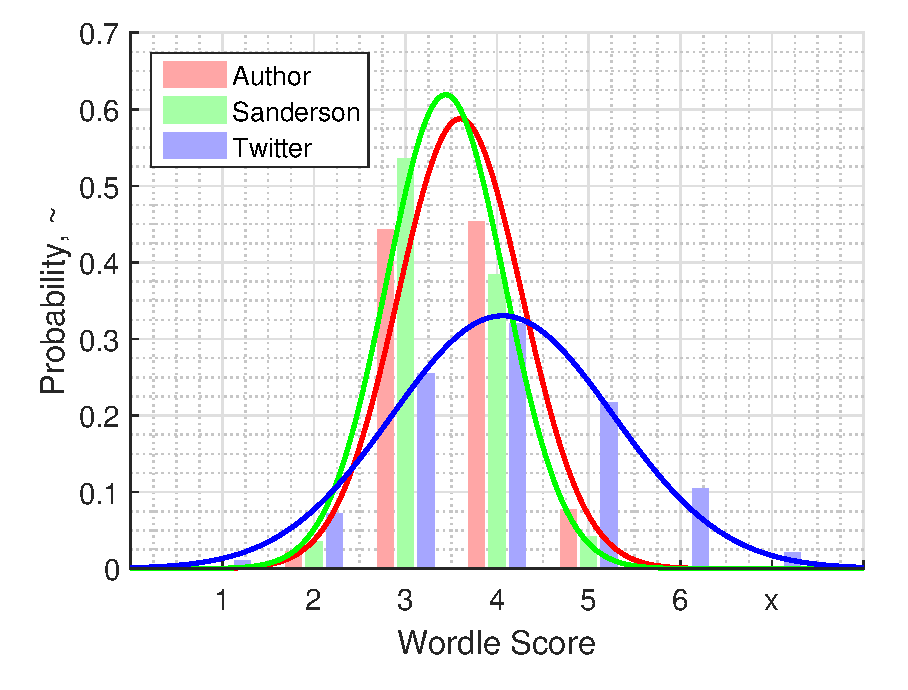
\includegraphics[width=0.5\textwidth]{performance_comparison.eps}
  \caption{Comparison of solver distributions. \rm Unassisted and current-best play are shown as limiting cases.}
\label{performance_comparison}
\end{figure}

%%%%% Bibliography %%%%%

%\renewcommand{\bibpreamble}{For a full documentation of the references, please refer to the sample.bib file. You can delete this text/command safely in main.tex at line 73. \cite{example-article,example-article-published-online,example-inbook,example-inbook-series-with-editor,example-inproceedings,example-proceedings,example-report,example-paper,example-phdthesis}}

\raggedright

\bibliography{article}

\begin{thebibliography}{9}

\bibitem{Wardle}
Wardle, Josh. \emph{Wordle - a daily word game.} Accessed February 6, 2022. https://www.powerlanguage.co.uk/wordle/.

\bibitem{Glaiel}
Glaiel, Tyler. \emph{The mathematically optimal first guess in Wordle.} Accessed February 6, 2022. https://medium.com/@tglaiel/the-mathematically-optimal-first-guess-in-wordle-cbcb03c19b0a.

\bibitem{WordleStats}
O'Connor, Kevin. \emph{Wordle Stats (@WordleStats) / Twitter.} Accessed February 6, 2022. https://twitter.com/wordlestats.

\bibitem{Dichter}
Dichter, Daniel. \emph{wordle\_solver.} Accessed February 6, 2022. https://github.com/kindofdoon/wordle\_solver.

\bibitem{Sanderson}
Sanderson, Grant. \emph{The mathematically optimal Wordle strategy.} 3Blue1Brown. Accessed February 6, 2022. https://www.youtube.com/watch?v=v68zYyaEmEA.

\bibitem{Chao}
Chao, Jason. \emph{Wordle-Solver.} Accessed February 6, 2022. https://github.com/jason-chao/wordle-solver.

\bibitem{Filion}
Filion, Adam. \emph{Building a Wordle Solver.} Accessed February 6, 2022. https://blogs.mathworks.com/loren/2022/01/18/building-a-wordle-solver/.

\end{thebibliography}

\end{document}













